%%%%%%%%%%%%%%%%%%%%%%%%%%%%%%%%%%%%%%%%%%%%%%%%%%%%%%%%%%
%                                                                                      %
%         Bristol Project LaTex Template            %
%                                                                                      %
%%%%%%%%%%%%%%%%%%%%%%%%%%%%%%%%%%%%%%%%%%%%%%%%%%%%%%%%%%
%
%   Author: Alex Charles           Email: aep.charles@gmail.com
%
% -----------------------------------------------------------------------------------
%      PACKAGES & OTHER DOCUMENT CONFIGURATIONS
% -----------------------------------------------------------------------------------
\documentclass[11pt]{article}
\usepackage[utf8]{inputenc}
\usepackage[T1]{fontenc}
\usepackage[british]{babel}
% ----------NEW BIBLATEX BIBLIOGRAPHY-----------------------------------------------
\usepackage[backend=bibtex,style = ieee]{biblatex} % Upgrades Bibliography

\addbibresource{BibFile.bib} %%% For biblatex
%e.g to add page number \footfullcite[chapter, p.~215]{AAIB}
% This allows can use footfullcite commands
% Note urldate field must be in yyyy-mm-dd to work - use online type
% Remeber to use \printbibliography in the footer
% -----------------------------------------------------------------------------------
\usepackage{sectsty}
\usepackage{amssymb,amsmath}
\usepackage{ifxetex,ifluatex}  %<<<<<<<<< Edit FONT HERE
\ifnum 0\ifxetex 1\fi\ifluatex 1\fi=0 % if pdftex
  \usepackage[T1]{fontenc}
  \usepackage[utf8]{inputenc}
\else % if luatex or xelatex
  \ifxetex
    \usepackage{mathspec}
    \setmainfont{Avenir-Light}
  \else
  % Font Package for XeLatex
    \usepackage{fontspec}
    \setmainfont{Avenir-Light}
  \fi
  \defaultfontfeatures{Ligatures=TeX,Scale=MatchLowercase}
\fi
\usepackage[fit]{truncate} %Truncates headers that are too long
\usepackage{fancyhdr}
\usepackage{lastpage}
\usepackage{extramarks}
\usepackage{gensymb}
\usepackage{lipsum}
\usepackage{float}
\usepackage{graphicx}
\graphicspath{{TempImg/}{Img/}}%<<<<<<<<< Location of Template Images and Other Images, Add folders here
\usepackage{subfig}
\usepackage{wrapfig}
\usepackage[font ={small,it}]{caption}
\usepackage{amsfonts,amsthm} % Math packages
% \usepackage{cite}
% \usepackage[maxlevel=3]{csquotes}
%    \MakeAutoQuote{‘}{’}
%    \MakeAutoQuote*{“}{”} %corrects quote marks
\usepackage{enumitem} % resume numbered lists
\usepackage{multicol} %for mulitple colums in lists
\usepackage{geometry}
\usepackage{booktabs} %<<<<<<<<< Table drawing package
\usepackage[table,xcdraw]{xcolor} %<<<<<<<<< Table drawing package
\usepackage{svg}
\usepackage{scrextend} %call footnotes
\usepackage[colorlinks, linkcolor = black, citecolor = black, filecolor = black, urlcolor = blue]{hyperref} % Creates Hyperlinks for references - add [colorlinks] for coloured hyperlinks
\usepackage{changepage} %Allows Adjust width to be used for the document (indenting paragraphs)
\usepackage{pdfpages} %Allows Pdfpages to be added to the document use \includepdf[pages={1}]{myfile.pdf}
\usepackage{pdflscape} %Change Pages from Portrait to Landscape

%\usepackage[compact]{titlesec}
\usepackage{titlesec}
\titlespacing\section{0pt}{2pt plus 2pt minus 2pt}{0pt plus 2pt minus 2pt}
\titlespacing\subsection{0pt}{0pt plus 3pt minus 2pt}{-3pt plus 2pt minus 2pt}
\titlespacing\subsubsection{0pt}{0pt plus 2pt minus 2pt}{-4pt plus 2pt minus 2pt}
\titlespacing\subsubsubsection{0pt}{-6pt plus 2pt minus 2pt}{-4pt plus 2pt minus 2pt}
\setlength{\multicolsep}{-1pt plus 2.0pt minus 1.5pt}% 50% of original values

% \titlespacing*{\section}{0pt}{1.1\baselineskip}{\baselineskip}

\renewcommand*{\thefootnote}{\alph{footnote}} %%% Changes footnotes to letters
\usepackage[bottom]{footmisc} %%% Pushes footnote to bottom and to the margin

\DeclareCiteCommand{\footcite}[\mkbibfootnote]
{\usebibmacro{cite:init}%
\usebibmacro{prenote}}
{\usebibmacro{citeindex}%
\printtext[brackets]{\usebibmacro{cite:comp}}}
{\multicitedelim}
{\usebibmacro{cite:dump}%
\usebibmacro{postnote}}

\newenvironment{indentpara}{\begin{adjustwidth}{2cm}{}}{\end{adjustwidth}} %Declare adjust width wiht indentpara
\renewcommand{\labelitemii}{$\circ$}
\renewcommand{\labelitemiii}{$\diamond$}
\renewcommand{\labelitemiii}{$\cdot$}

% -----------------------------------------------------------------------------------
%                 Code
% -----------------------------------------------------------------------------------
\usepackage{listings}
\lstset{inputpath=Code/}
\usepackage{color}
\definecolor{mygreen}{RGB}{28,172,0} % color values Red, Green, Blue
\definecolor{mylilas}{RGB}{170,55,241}

\lstset{language=Matlab,%
    %basicstyle=\color{red},
    breaklines=true,%
    basicstyle=\small,
    morekeywords={matlab2tikz},
    keywordstyle=\color{blue},%
    morekeywords=[2]{1}, keywordstyle=[2]{\color{black}},
    identifierstyle=\color{black},%
    stringstyle=\color{mylilas},
    commentstyle=\color{mygreen},%
    showstringspaces=false,%without this there will be a symbol in the places where there is a space
    numbers=left,%
    numberstyle={\tiny \color{black}},% size of the numbers
    numbersep=9pt, % this defines how far the numbers are from the text
    emph=[1]{for,end,break},emphstyle=[1]\color{red}, %some words to emphasise
    %emph=[2]{word1,word2}, emphstyle=[2]{style},
}

%% To Add Code Use :
% \lstinputlisting{myfun.m}
%% To input a file or :
% \begin{figure}[h]
% \begin{lstlisting}[language=Matlab]
% \end{lstlisting}
% \catpion{code}
% \end{figure}


% -----------------------------------------------------------------------------------
%                 Quotes
% -----------------------------------------------------------------------------------

\usepackage{epigraph}
% \epigraphsize{\small}% Default
\setlength\epigraphwidth{12cm}
\setlength\epigraphrule{0pt}

\usepackage{etoolbox}
\apptocmd{\sloppy}{\hbadness 10000\relax}{}{}%%%% > Removes Url bibliography warnings
\makeatletter
\patchcmd{\epigraph}{\@epitext{#1}}{\itshape\@epitext{#1}}{}{}
\makeatother

%%%% > For Quotes Use \epigraph{"Quote"}{ - \textup{Author}, Book}

% -----------------------------------------------------------------------------------
%                   NAMES & CLASS DEFINITION %<<<<<<<<< INSERT DETAILS HERE
% -----------------------------------------------------------------------------------
\newcommand{\AssignmentTitle}{Part 3: PID Implementation, Validation and Retuning in Quanser}
\newcommand{\ModuleTitle}{Sensors, Signals and Control}
\newcommand{\University}{University of Bristol}
\newcommand{\Faculty}{Faculty of Engineering}
\newcommand{\UniCrest}{crestbris.png}
\newcommand{\UniLogo}{logobris.png}%<<<<<<<<< Make Sure Files are in the Template
%\newcommand{\GroupName}{Group 2}
\newcommand{\StudentNameA}{Alex Charles}
\newcommand{\StudentNumberA}{ac13625}
\newcommand{\StudentNameB}{Akash Ramineni}
\newcommand{\StudentNumberB}{ar14120}
\newcommand{\SupervisorNameA}{Andres Marcos}
\newcommand{\SupervisorEmailA}{Andres.Marcos@bristol.ac.uk}
\newcommand{\SupervisorNameB}{Name}
\newcommand{\SupervisorEmailB}{email@gmail.com}

% -----------------------------------------------------------------------------------
%        PACKAGES FOR MARKDOWN CONVERSION - FOR USE If Using Markdown to Latex
% -----------------------------------------------------------------------------------
\usepackage{fixltx2e} % provides \textsubscript
% use upquote if available, for straight quotes in verbatim environments
\IfFileExists{upquote.sty}{\usepackage{upquote}}{}
% use microtype if available
\IfFileExists{microtype.sty}{%
\usepackage{microtype}
\UseMicrotypeSet[protrusion]{basicmath} % disable protrusion for tt fonts
}{}
\hypersetup{unicode=true,
            pdftitle={\AssignmentTitle},
            pdfauthor={\StudentNameA},
            pdfborder={0 0 0},
            breaklinks=true}
\urlstyle{same}  % don't use monospace font for urls
\usepackage{fancyvrb}
\VerbatimFootnotes % allows verbatim text in footnotes
\usepackage{longtable,booktabs}
\IfFileExists{parskip.sty}{%
\usepackage{parskip}
}{% else
\setlength{\parindent}{0pt}s
\setlength{\parskip}{6pt plus 2pt minus 1pt}
}
\setlength{\emergencystretch}{3em}  % prevent overfull lines
\providecommand{\tightlist}{%
  \setlength{\itemsep}{0pt}\setlength{\parskip}{0pt}}
% \setcounter{secnumdepth}{0}
% Redefines (sub)paragraphs to behave more like sections
\ifx\paragraph\undefined\else
\let\oldparagraph\paragraph
\renewcommand{\paragraph}[1]{\oldparagraph{#1}\mbox{}}
\fi
\ifx\subparagraph\undefined\else
\let\oldsubparagraph\subparagraph
\renewcommand{\subparagraph}[1]{\oldsubparagraph{#1}\mbox{}}
\fi

% -----------------------------------------------------------------------------------
%                   WORD COUTNER - for XeLaTex
% -----------------------------------------------------------------------------------
\usepackage{xesearch}
\newcounter{words}
\newenvironment{counted}{%
  \setcounter{words}{0}
  \SearchList!{wordcount}{\stepcounter{words}}
    {a?,b?,c?,d?,e?,f?,g?,h?,i?,j?,k?,l?,m?,
    n?,o?,p?,q?,r?,s?,t?,u?,v?,w?,x?,y?,z?}
  \UndoBoundary{'}
  \SearchOrder{p;}}{%
  \StopSearching}

% -----------------------------------------------------------------------------------
%                   MARGINS, HEADERS & FOOTERS
% -----------------------------------------------------------------------------------
 \geometry{
 left=20mm,
 right=20mm,
 top=20mm,
 bottom=20mm,
 }
\linespread{1.05}

\pagestyle{fancy}
\lhead{\includegraphics[width = 0.2\textwidth]{\UniLogo}}
% \chead{\AssignmentTitle}
% \rhead{}
\lfoot{\StudentNameA, \StudentNameB}
\cfoot{}
\rfoot{Page \thepage} %%%% note the footer is swapped when page numbering style changes
\renewcommand\headrulewidth{0.4pt}
\renewcommand\footrulewidth{0.4pt}

\setlength\parindent{0pt}

\newcommand{\horrule}[1]{\rule{\linewidth}{#1}}

% -----------------------------------------------------------------------------------
%               DOCUMENT STRUCTURE COMMANDS
% -----------------------------------------------------------------------------------
% To sort out the formatting of header and footer when a page...
% ... split occurs "within" a problem environment.
\newcommand{\enterProblemHeader}[1]{
\nobreak\extramarks{#1 (Cont.)}\nobreak
\nobreak\extramarks{#1}{}\nobreak
}
% To sort out the formatting of header and footer when a page...
% ... split occur "between" problem environments.
\newcommand{\exitProblemHeader}[1]{
\nobreak\extramarks{#1 (Cont.)}\nobreak
\nobreak\extramarks{#1}{}\nobreak
}

% -----------------------------------------------------------------------------------
\begin{document}

  \setlength{\abovedisplayskip}{-14pt}
  \setlength{\belowdisplayskip}{2pt}
  \setlength{\abovedisplayshortskip}{-14pt}
  \setlength{\belowdisplayshortskip}{2pt}

  \setlist[enumerate]{itemsep=-2mm}
  \setlist[itemize]{itemsep=-2mm}


%----------------------------------------------------------------------------------------
                                  %	TITLE PAGE FORMAT
%----------------------------------------------------------------------------------------
\pagenumbering{roman}
\begin{titlepage}

	\center % Center everything on the page
%----------------------------------------------------------------------------------------
%	HEADING SECTION
%----------------------------------------------------------------------------------------
		\usefont{OT1}{bch}{b}{n}
		\normalfont \normalsize \textsc{\University} \\ [10pt]
		\normalfont \normalsize \textsc{\Faculty} \\ [25pt]
%----------------------------------------------------------------------------------------
%	LOGO SECTION - Adds Univeristy Crest to the Report
%----------------------------------------------------------------------------------------
		\includegraphics[width = 0.2\textwidth]{\UniCrest}\\[0.5cm]
%----------------------------------------------------------------------------------------
%	HEADING SECTION
%----------------------------------------------------------------------------------------
		\normalfont \normalsize \textsc{\ModuleTitle} \\ [25pt]
%----------------------------------------------------------------------------------------
%	TITLE SECTION
%----------------------------------------------------------------------------------------
		\horrule{0.5pt} \\[0.4cm]
		\huge \textbf{\AssignmentTitle} \\
		\horrule{2pt} \\[0.5cm]
%----------------------------------------------------------------------------------------
%	HEADING SECTION
%----------------------------------------------------------------------------------------
%		\normalfont \normalsize \textsc{\GroupName} \\ [25pt]
%----------------------------------------------------------------------------------------
%	AUTHOR SECTION
%----------------------------------------------------------------------------------------
\begin{minipage}{0.4\textwidth}
\begin{flushleft} \large
\emph{Supervisors:}\\
% Change Name
\textbf{\SupervisorNameA}\\
% \textbf{\SupervisorNameB}
\end{flushleft}
\end{minipage}
~
\begin{minipage}{0.4\textwidth}
\begin{flushright} \large
\emph{Email:} \\
\SupervisorEmailA\\
% \SupervisorEmailB

\end{flushright}
\end{minipage}\\[1cm]

\begin{minipage}{0.4\textwidth}
\begin{flushleft} \large
\emph{Authors:}\\
	\textbf{\StudentNameA}\\
  \textbf{\StudentNameB}
\end{flushleft}
\end{minipage}
~
\begin{minipage}{0.4\textwidth}
\begin{flushright} \large
\emph{Candidate Number:} \\
(\StudentNumberA)\\
(\StudentNumberB)
\end{flushright}
\end{minipage}\\[2cm]

%----------------------------------------------------------------------------------------
%	DATE SECTION
%----------------------------------------------------------------------------------------
\textit{{\large \today}}\\[1cm] % Date, change the \today to a set date if you want to be precise
%----------------------------------------------------------------------------------------
\vfill % Fill the rest of the page with whitespace
\end{titlepage}

% \setcounter{page}{3}

\newpage


% -----------------------------------------------------------------------------------
%                             	 ABSTRACT
% -----------------------------------------------------------------------------------

% \addcontentsline{toc}{section}{Abstract}
% \begin{abstract}
%
% \end{abstract}
% -----------------------------------------------------------------------------------
%                              TABLE OF CONTENTS
% -----------------------------------------------------------------------------------

% \tableofcontents


% \newpage

% \addcontentsline{toc}{section}{List of Tables}
% \listoftables
% \addcontentsline{toc}{section}{List of Figures}
% \listoffigures
% \addcontentsline{toc}{section}{List of Acronyms}
% \section*{List of Acronyms}\label{acronyms}
% \textbf{BRB}: Be Right Back \\


% \newpage

% \addcontentsline{toc}{section}{Acknowledgements}
% \section*{Acknowledgements}\label{acknowledgements}

% \addcontentsline{toc}{section}{Declaration}
% \section*{Declaration}\label{declartion}
% I hereby declare that this report entitled “\AssignmentTitle” submitted to Bristol University, is a record of an original work completed by myself.\\

% \newpage

%% -----------------------------------------------------------------------------------
%%                          	  INTRODUCTION
%% -----------------------------------------------------------------------------------
\clearpage
\rfoot{Page \thepage\ of \pageref{LastPage}}
\pagenumbering{arabic}
\begin{counted} %<<<<<<<<<<<<<<STARTS WORD COUNTER
\section{Introduction}\label{introduction}

This report analyses the effectiveness of a using a PID controller
derived in Phase 2 on a Quanser-rig. Before implementing the controller
on the Quanser-rig, nonlinearities in the form of a rate limiter and
saturation were added to the simulation. By implementing a design
process, new control objectives were met, then implemented on the
Quanser-rig The following report discusses both the design process,
results and any observations made through creating an effective
controller for the Quanser-rig.

The following transfer function was used to design the controller, taken
from Phase 1:

\begin{align*}
&\text{$2^{nd}$ Order: }k \cdot \frac { 1.109\cdot \frac{180} {\pi} }{ s^2 + 0.1313s +1.109 }
&&\text{$1^{st}$ Order: }k \cdot \frac { 1 }{ 15.24s +1 }
\end{align*}

Where \(k = 0.26\).

\section{Nonlinearity Simulation Control
Refinement}\label{nonlinearity-simulation-control-refinement}

\begin{wrapfigure}{r}{0.4\textwidth}
 \vspace{-25pt}
 \centering
  \includegraphics[trim = 0 0 0 0, clip, width=0.395\textwidth]{origcontrol.pdf}
\vspace{-10pt}
  \caption{Showing original Controller Architecture}
  \vspace{-25pt}
  \label{origcontrol}
 \end{wrapfigure}

In Quanser Control Part 3, the improved PID controller successfully met
the Phase 2 requirements but failed to meet the overshoot (OS) condition
for the refined controller. The PID control architecture in Figure
\ref{origcontrol} from Part 2 was tested using both non-linear
simulation and on the Quanser setup.

\begin{wrapfigure}{r}{0.4\textwidth}
 \vspace{-25pt}
 \centering
  \includegraphics[trim = 0 0 0 0, clip, width=0.395\textwidth]{fincontrol.pdf}
\vspace{-10pt}
  \caption{Showing Improved Controller Architecture}
  \vspace{-20pt}
  \label{fincontrol}
 \end{wrapfigure}

At this stage, the design process for the controller consisted of;
extracting preliminary responses from the Quanser-rig, analysing the
responses to obtain a simulated plant transfer function. The transfer
function was designed to represent small changes in elevation angle,
whereby purely tuning the gains, manifested a desirable response. The
controller, therefore, was built to achieve a good response in the
simulation, so is susceptible to errors when translating to the real
Quanser-rig.

For the controller to meet the overshoot requirement, the controller was
further refined in the simulation. Through using understanding taken
from Phase 2, shown in Table \ref{paramtab}, gains were modified to
improve the results further. Starting with the integrator gain
(\(K_i\)), which had the greatest effect on reducing the steady-state
error, this was increased by an increment, until the transfer function
response began to deteriorate. \(K_i\) had only a small range in which
the response could be altered without degrading the results; suggesting
that the original \(K_i\) value was a good fit. Maximising \(K_i\)
first, meant that the effects of varying derivative gain (\(K_d\)) on
the steady state would be minimised. A similar process was followed for
then the proportional gain (\(K_p\)) and \(K_d\), where \(K_p\) was
maximised to reduce the rise time (\(T_R\)) and \(K_d\) was optimised to
reduce the overshoot \(OS\). Maximising these values, helped improve the
performance characteristics without heavily deteriorating other
properties.

\begin{wrapfigure}{l}{0.42\textwidth}
 \vspace{-25pt}
\centering
\captionof{table}{Effect of Increasing PID Gains on Objectives}
\vspace{-5pt}
 \includegraphics[trim = 0 0 0 0, clip, width=0.419\textwidth]{tableobj.pdf}
 \vspace{-25pt}
 \label{paramtab}
 \end{wrapfigure}

To test the controller performance more vigorously, the PID was run in a
new simulation, with non-linearities added; in the form of a rate
limiter and saturation block. A rate limiter block limits the speed of
change of the signal, and the saturation represents a limit in
amplitude. This new simulation would improve the accuracy of emulation
to expected Quanser response. A marginal change could be seen when
comparing the results of the non-linear simulation to the original,
where overshoot would increase slightly. Further experimentation found
that increasing gain values by an order of magnitude, destabilised the
results revealing much greater non-linear effects; further confirming
that the PID gains selected, fell within an acceptable region. With a
small additional tweaking following the same design process, the final
gain values are shown in in Table \ref{gains} met the requirements of
the Phase 3 design characteristics.

\begin{wrapfigure}{r}{0.255\textwidth}
\vspace{-30pt}
 \centering
  \captionof{table}{Showing Controller Gain Values Used}
 \includegraphics[trim = 0 0 0 0, clip, width=0.254\textwidth]{gains2.pdf}
 \label{gains}
\vspace{-20pt}
 \end{wrapfigure}

Figure \ref{fincontrol} shows the original controller configuration
utilised the numerical Simulink derivative block within the PID
controller. It was found that the control architecture could also be
improved for the actual control rig. Using the derivative as output
directly \texttt{y\_elevdot} from the Quanser - it was expected that the
numerical derivative block would not be as representative of the
observed rate of change as the actual derivative output. This view was
confirmed by the improved experimental results from provisional testing
on the Quanser-Rig. The difference in architecture was unobservable in
simulation, highlighting a noticeable difference between real and
simulated output data.

\section{Quanser Controller
Refinements}\label{quanser-controller-refinements}

After satisfying the desired requirements in the non-linear simulation,
the controller tests were conducted on the Quanser-rig. The controller
performed well, meeting the desired requirements, where a small
improvement in overshoot could be observed from the simulation. Due
sampling errors small deviations from the steady state could be seen
(see \ref{quanscomp}) of \(\pm 0.4\)\% could be seen from elevation
angle. As the sampling rate was limited by the sensors on the Quanser,
results appeared jagged, reducing the precision of the results; this was
small enough, results to be accurate enough at representing the response
of the Quanser.

\section{Results}\label{results}

\begin{figure}[H]
 \centering
 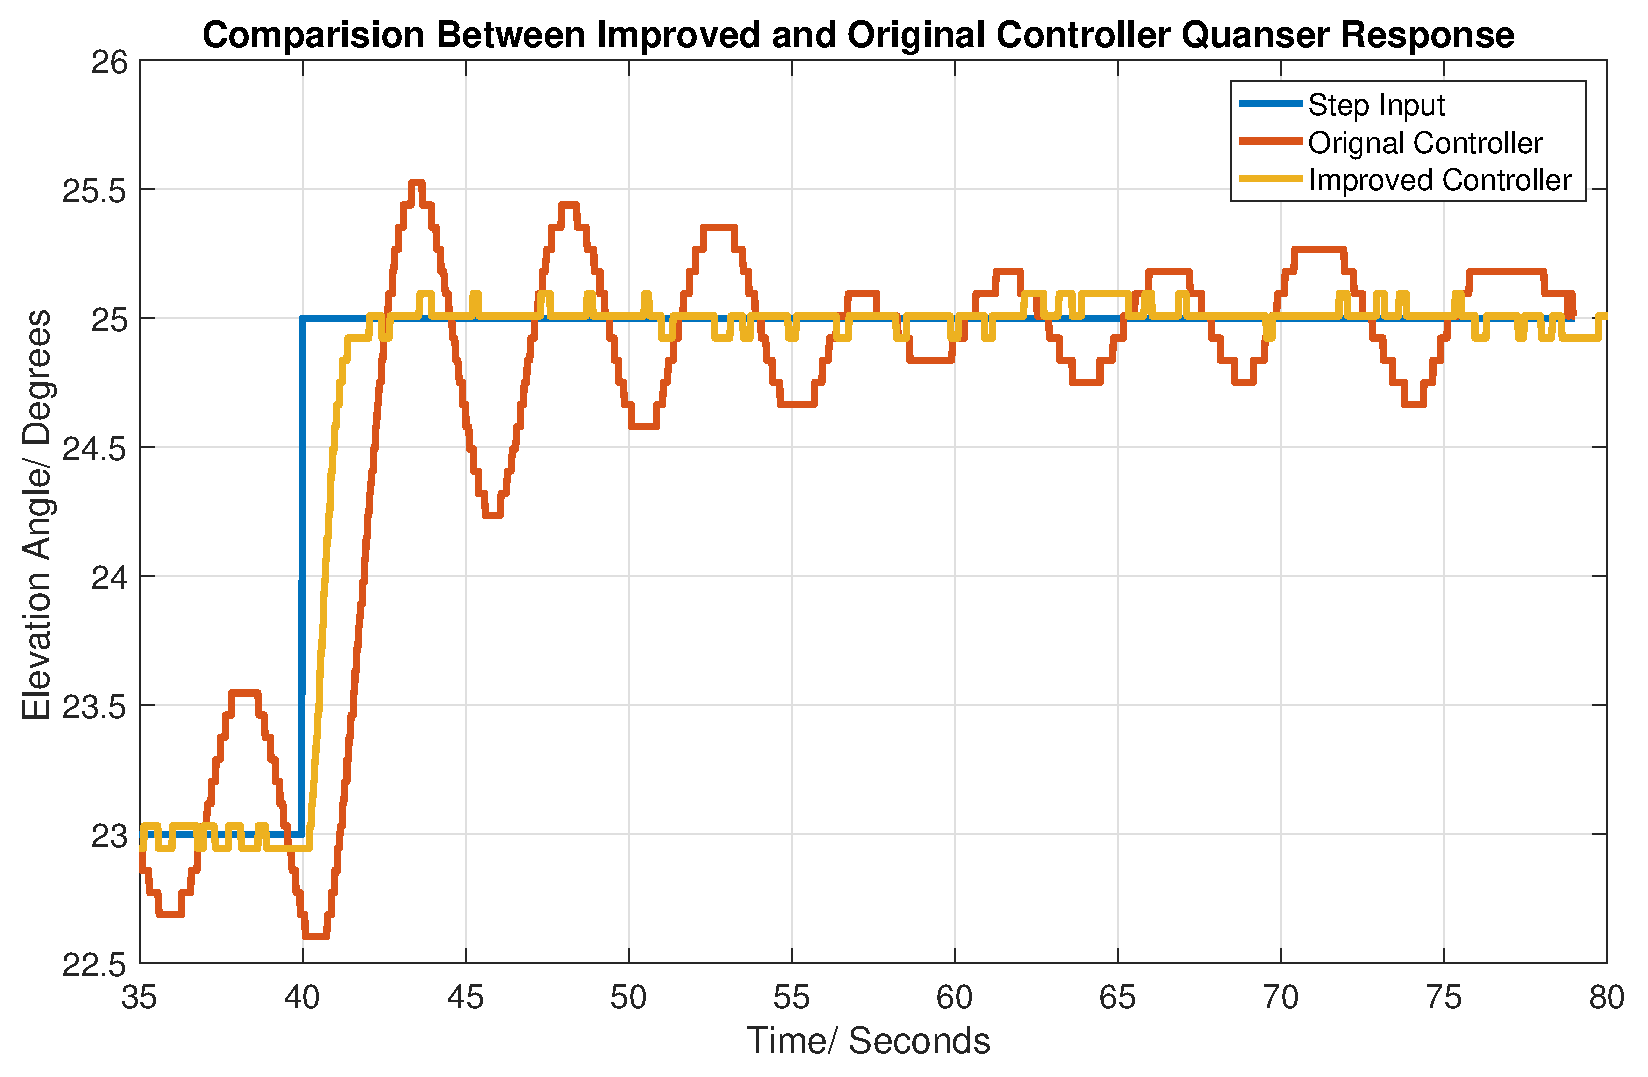
\includegraphics[trim = 0 0 0 0, clip, width=0.6\textwidth]{quanscomp.eps}
\caption{Showing Difference in Original and Improved Controller Performance on Quanser Response}
 \label{quanscomp}
 \end{figure}

\begin{figure}[H]
\centering
\begin{minipage}{.49\textwidth}
\centering
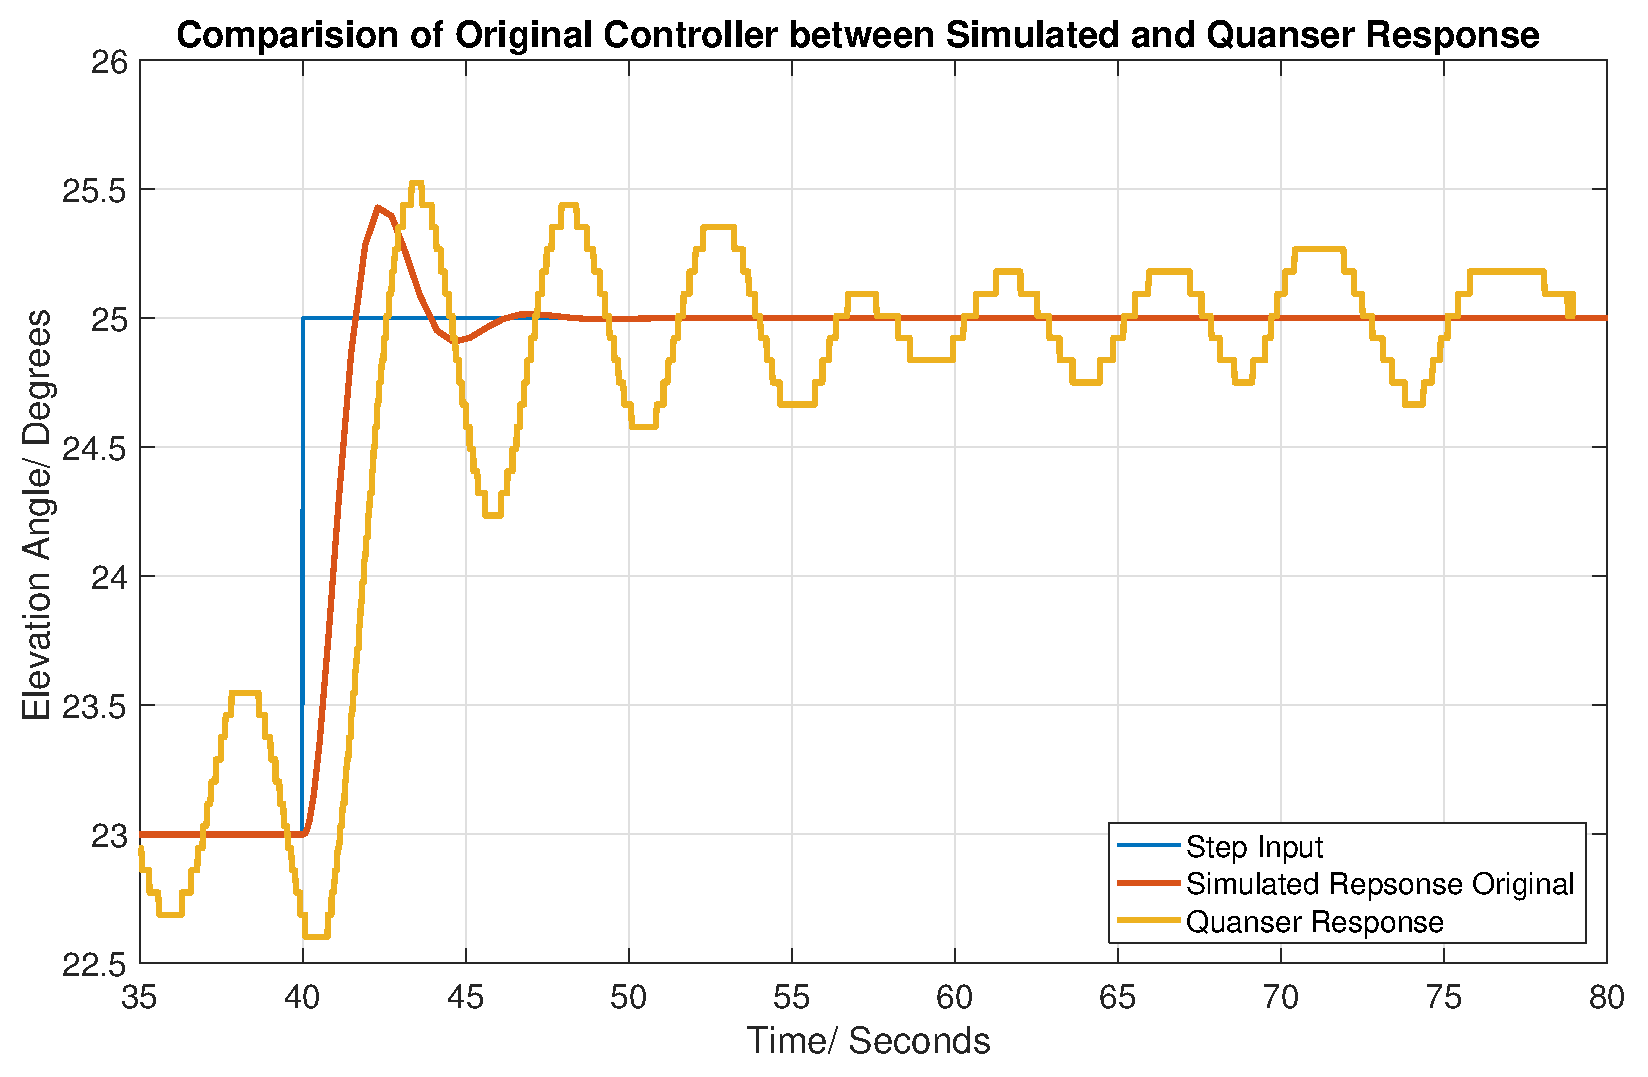
\includegraphics[trim = 0 0 0 0, clip, width=1\textwidth]{origresult.eps}
\caption{Showing Difference in Original Controller Performance Comparing Simulated and Quanser Responses}
\label{origresult}
\end{minipage}
\hfill
\begin{minipage}{.49\textwidth}
\centering
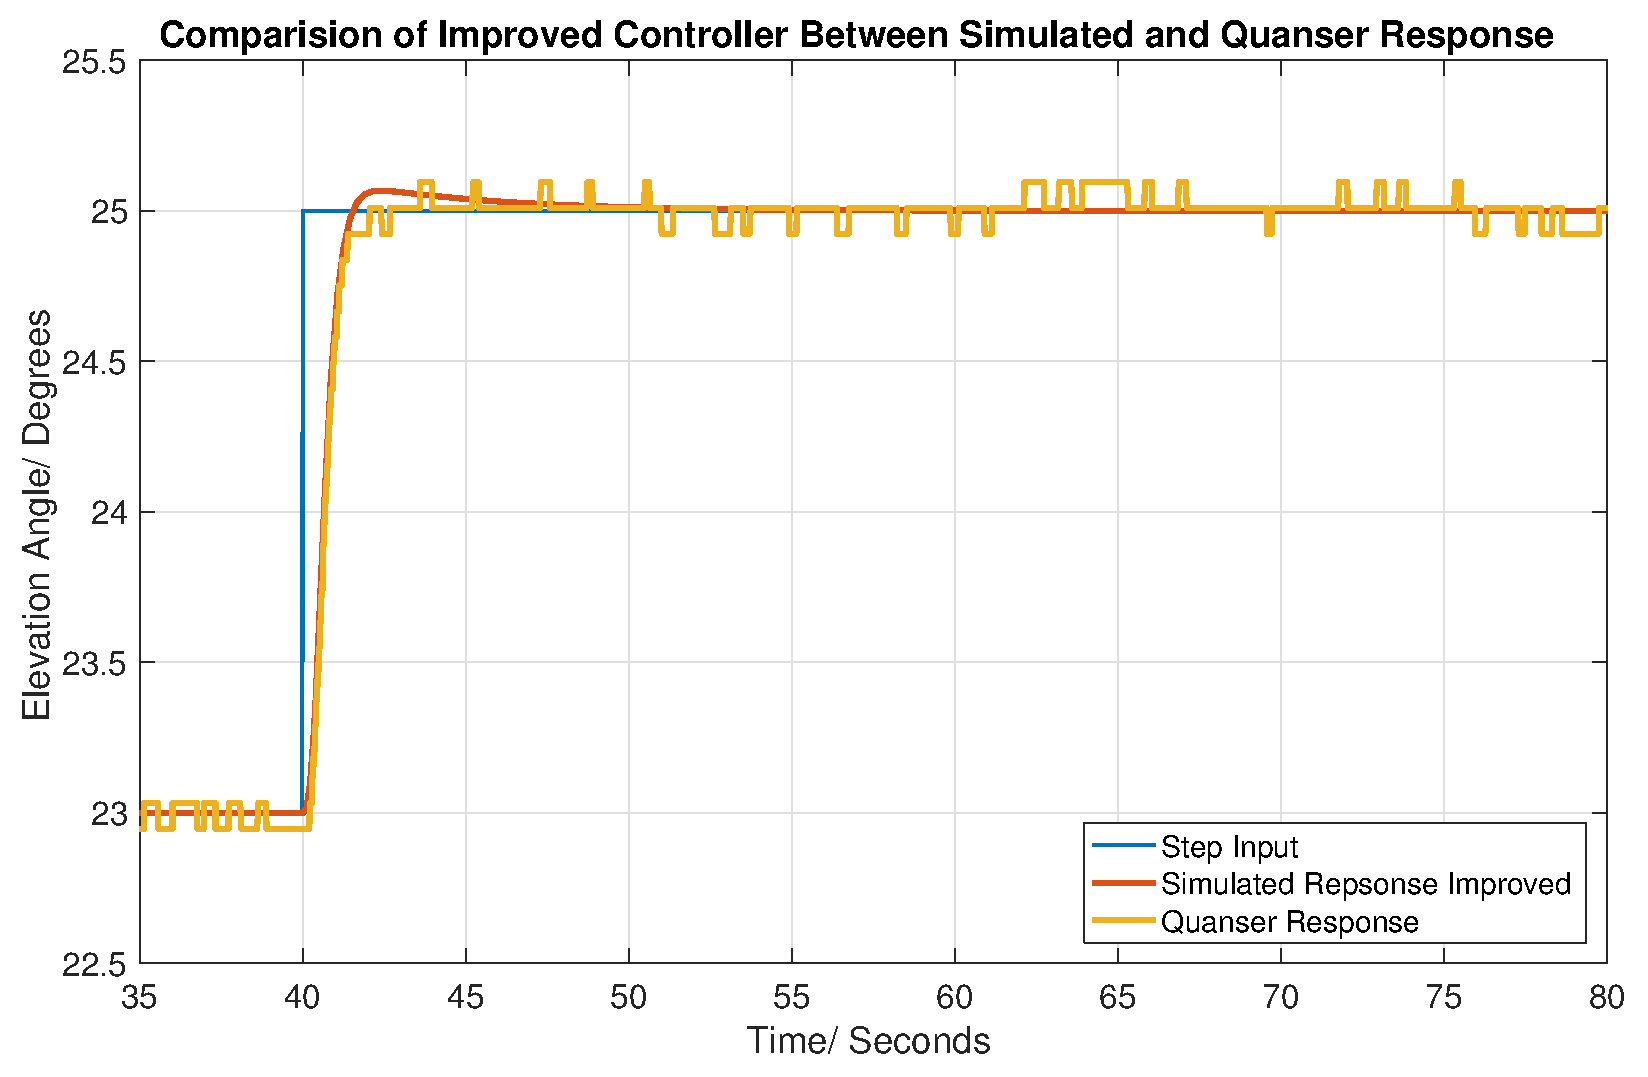
\includegraphics[trim = 0 0 0 0, clip, width=1\textwidth]{improvresult.eps}
\caption{Showing Difference in Improved Controller Performance Comparing Simulated and Quanser Responses}
\label{improvresult}
\end{minipage}
\vspace{-20pt}
\end{figure}

\begin{table}[H]
 \centering
 \caption{Showing Controller Response Results for Simulation and Quanser Tests}
 \includegraphics[trim = 0 0 0 0, clip, width=0.65\textwidth]{resultstab2.pdf}
 \label{resultstab}
 \end{table}

\section{Discussion}\label{discussion}

Figure \ref{quanscomp} highlights the experimental difference between
the original tuned PID controller (taken directly from Part 2) and the
iteratively improved, (with an alternative architecture ) PID
controller. The improved Quanser response displayed a rise time of 2.18
seconds, settling time of 2.18 seconds (as the 4\% error limits were
satisfied at the same time as the rise time), an Overshoot of 0.48\% and
a negligible steady state error. These values comfortably satisfied the
required objectives and also improving upon the desired objectives shown
in Table \ref{resultstab}. The improved controller showed a faster rise
time, settling time and reduced overshoot \% over the original
controller design. In an engineering context, it is critical that the
controller response is sharp and responsive, minimising delay times.
Observing the step input time in Figure \ref{quanscomp}, it is evident
that the choice of the controller effects the delay/error when the Step
response. The Quanser was allowed to settle to a reasonable level before
the step input was tested, but the original controller showed larger
settling oscillations, this likely contributed towards the amplitude and
phase error displayed in \ref{origresult} between the simulated Quanser
response and the experimental Quanser response. This observation is also
reinforced by Figure \ref{improvresult} as the Simulink step input shows
less delay. Errors introduced from oscillations never settling
completely, also imply that when the step was applied, the response was
likely mid oscillations, adding the step response. This effect is likely
to be present in real world rotatory wing aircraft; the design
parameters were estimated conservatively to meet the requirements in any
case.

The idealisation of the elevator actuation could also be observed when
comparing the simulation to real world response. It was assumed that no
physical limitations are in place on the system. Realistically, this may
be misrepresenting the physical actuator, likely introducing errors in
the form of actuator delay.

The results presented above highlight the step response for the tuned
PID controller for a step input of, chosen as the transfer function was
derived from experimental results of elevator angle step changes between
-2 and 2. It is expected that for step inputs out of this range, the
tuned controller will perform sub-optimally; accurate near the
`fix-point' and showing deviations at higher step inputs.

\begin{wrapfigure}{r}{0.45\textwidth}
\vspace{-10pt}
\centering
 \includegraphics[trim = 0 0 0 0, clip, width=0.45\textwidth]{ampresmark.pdf}
\vspace{-5pt}
\caption{Showing Magnitude of Rate Response}
 \vspace{-20pt}
 \label{ampres}
\end{wrapfigure}

The Quanser experiment was set in a reasonably controlled `lab'
environment with few assumed non-linearities, and hence the PID was
designed with the assumption of weak non-linearities. A simple tuning
process was only needed to meet the specified requirements, which
resulted in a good response. In more complex engineering applications,
the system in question may display a larger number of non-linear
effects. This may be accounted for using the method of gain scheduling.
Gain Scheduling \cite{stackcont} achieves control of a non-linear system
by linearising the problem at various operation states; resulting in a
``family'' of PID controllers which will each respectively activate when
a certain operation state is achieved. Each of these PID controllers
must be tuned independently to optimise for their respective
linearisation. The design then switches between each of these models to
achieve the ``best response'' for the current state. More conclusively,
within limits of this study, the obtained tuned PID controller for the
Quanser is effective and meets the desired time domain requirements. For
further accuracy of either Quanser control or more complex systems;
additional control structures should be considered, particularly if the
controller should encompass less stable operations such as take-off and
landing.

In an aircraft control context, the control parameters may be altitude
or Mach.

\section{Conclusions}\label{conclusions}

This experiment has been a useful exercise in illustrating methods and
common pitfalls when transferring a theoretically functioning tuned PID
controller to a real world system. Predicting the Quanser response using
a non-linear simulation, allows for a good controller to be created but
exact characteristics are difficult to predict without real
experimentation and testing. Further controller refinement is therefore
required when transferring to the real system, using the simulation as a
method of getting close to the answer. It was interesting to note that
the real world response always varied from the expected simulations for
every tested tuned PID controller and configuration - this difference is
likely an artefact of the non-linearities present in the Quanser-rig.
% -----------------------------------------------------------------------------------
%                                  APENDIX
% -----------------------------------------------------------------------------------

\end{counted} %<<<<<<<<<<<<<<ENDS WORD COUNTER

% \newpage
% % \section{Appendices}
% Above were \thewords\ words. %<<<<<<<<<<<<<<DISPLAYS WORD COUNTER
% -----------------------------------------------------------------------------------
%                               BIBLIOGRAPHY - Insert Name of BIB File Here
% -----------------------------------------------------------------------------------
% \newpage

% ---------------BIBTEX OLD-----------------------------------------------------
% \bibliographystyle{unsrt} %%%% Plain or alpha can change orders here
% \bibliography{BibFile}
% \nocite{*} %%%if you want to see all references even those note cited in the text
% -----------------------------------------------------------------------------------

\printbibliography

\end{document}
